\documentclass{beamer}

%%%%%%%%%%%%%Solarized Theme%%%%%%%%%%%%%%%
\usecolortheme[dark,accent=cyan]{solarized}
\beamertemplatenavigationsymbolsempty
%%%%%Packages%%%%%
\usefonttheme{serif}
\usepackage[T1]{fontenc}
\usepackage[utf8]{inputenc}
\usepackage[english]{babel}
\usepackage{fontawesome}
\usepackage{minted}
\usepackage{soul}

\definecolor{DarkGray}{gray}{0.1}
\usemintedstyle{paraiso-dark}


\usepackage{graphicx}
\usepackage{hyperref}
\usepackage{colortbl, xcolor}
\usepackage{booktabs}
\usepackage{amsmath,amsthm, amssymb, latexsym}

\usepackage{tikz}
\usepackage{xcolor}
\usepackage{graphicx,multirow}
\definecolor{plain}{rgb}{93,93,93}
\usetikzlibrary{positioning,arrows}
\definecolor{applegreen}{rgb}{0.55, 0.71, 0.0}
\usetikzlibrary{decorations.pathreplacing, backgrounds, fit}
\usetikzlibrary{calc,matrix}

\tikzstyle{background}=[solarizedRed, rectangle, draw, inner sep=1mm, thick,
           rounded corners=2mm]

\usepackage{standalone}
\usepackage{siunitx}

\begin{document}

\begin{frame}
    \begin{center}
        \Large{\textcolor{orange}{\textcolor{orange}{Publishing and Citing open research code \\ Open Life Science}}} \\

        \vspace{1cm}
        \normalsize{@NikoletaGlyn}

    \end{center}
\end{frame}

\begin{frame}
    \begin{center}
    
\includegraphics[width=0.24\textwidth]{static/mpi.jpg}\hspace{8pt}
    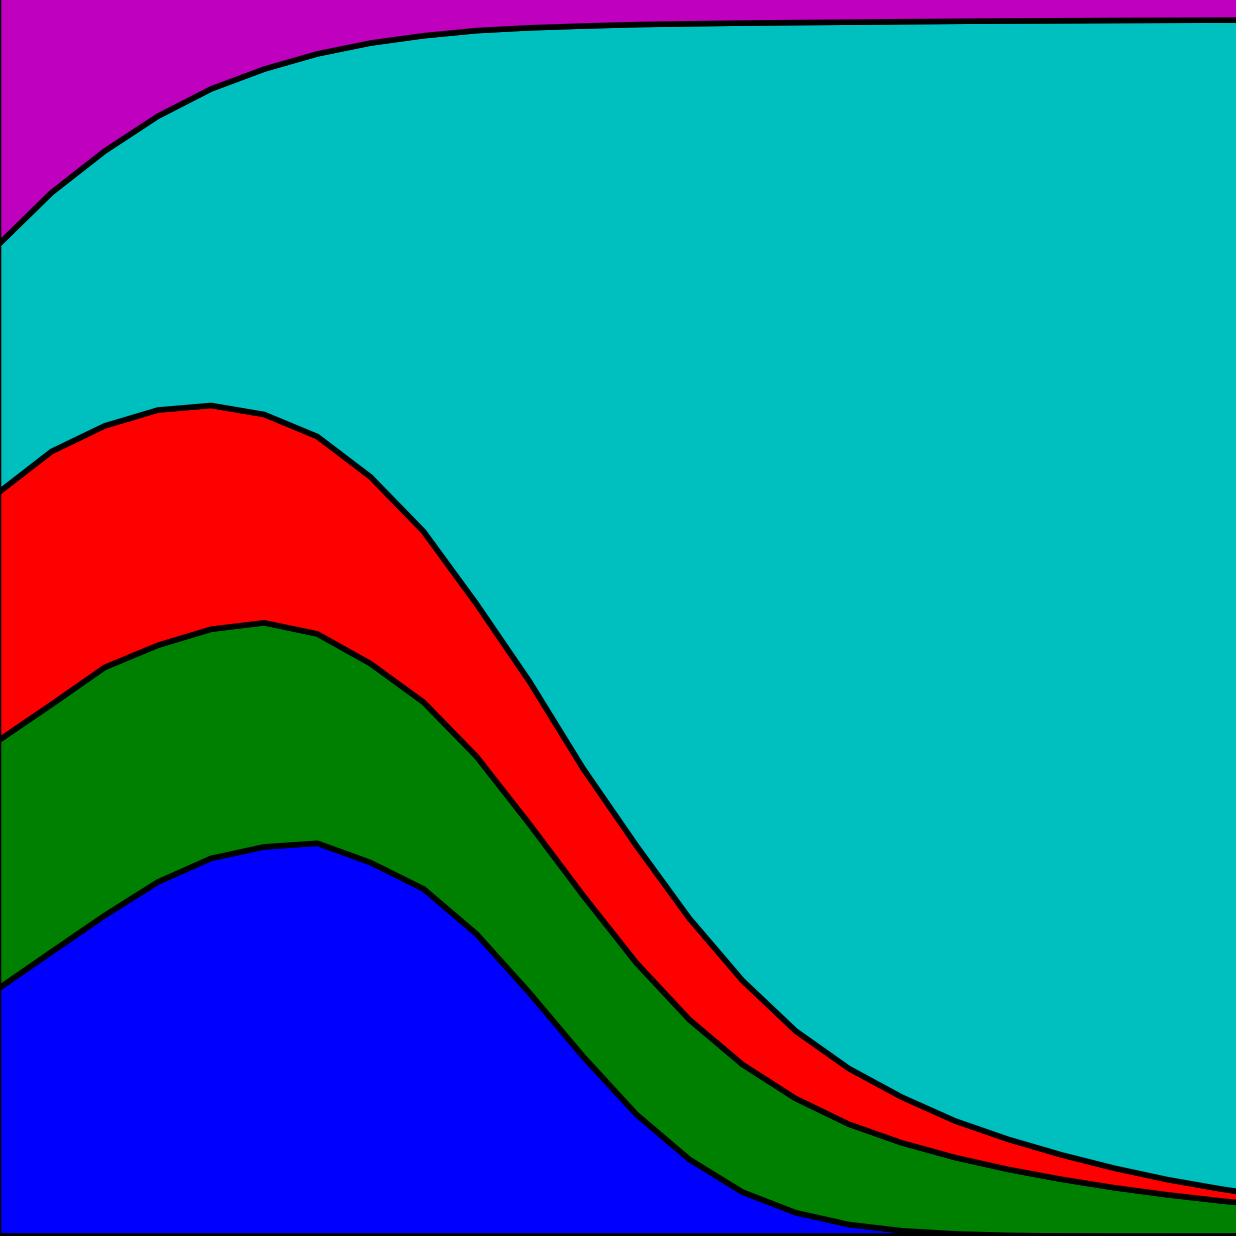
\includegraphics[width=0.24\textwidth]{static/axelrod-logo.png}\vspace{8pt}

    
\includegraphics[width=0.24\textwidth]{static/ssi-logo.png}\hspace{8pt}
    
\includegraphics[width=0.24\textwidth]{static/JOSS.png}
    \end{center}
\end{frame}

\begin{frame}
    \begin{center}
    
\includegraphics[width=\textwidth]{static/research_and_software.jpg}\hspace{8pt}
    \end{center}
\end{frame}

\begin{frame}
    \centering
    \Large{\textbf{\textcolor{orange}{Impossible to conduct research without software}}} \\
    \vspace{.3cm}

    \LARGE{\textbf{\textcolor{orange}{7/10 UK researchers}}}
    \vspace{2cm}

    \tiny{https://www.software.ac.uk/blog/2014-12-04-its-impossible-conduct-research-without-software-say-7-out-10-uk-researchers}
\end{frame}

\begin{frame}
    \centering
    \Large{\textbf{\textcolor{orange}{Why do we publish our} software\textcolor{orange}{?}}}
\end{frame}

% \begin{frame}
%     \centering
%     \Large{\textbf{\textcolor{orange}{Why do we publish our} \st{software}\textcolor{orange}{?}}}
% \end{frame}


\begin{frame}
    \centering
    \Large{\textbf{\textcolor{orange}{Why do we publish our} research output?}}
\end{frame}

\begin{frame}
    \textbf{
    \begin{itemize}
        \item increase visibility of our work
        \item easily quantifiable recognition and credit through e.g. citation counts
        \item peer review process should lead to better quality output
    \end{itemize}}
\end{frame}

\begin{frame}
    \begin{center}
    
\includegraphics[width=0.25\textwidth]{static/office-building.png}\hspace{20pt}
    \pause
    
\includegraphics[width=0.25\textwidth]{static/woman-technologist.png}
    \end{center}
\end{frame}

% \begin{frame}
%     \begin{center}
%         \small
%     \faTwitter \ @NikoletaGlyn \\
%     \faGithub \ \url{https://github.com/Nikoleta-v3} \\
%     \faGithub \ \url{https://github.com/Nikoleta-v3/avengers-analysis} \\ \vspace{1cm}



%     \tiny{\url{https://medium.com/swlh/avengers-web-scraping-entity-extraction-and-network-graphs-in-python-ea6dc323eb7d}}
%     \end{center}
% \end{frame}

\end{document}